\newif\ifsolutions
\solutionstrue % Show solutions
%\solutionsfalse % Hide solutions

\documentclass{article}
\usepackage{geometry}
\geometry{margin=1in}
\usepackage{tikz}
\usepackage{amssymb}

% fleqn allows setting indent of display math
\usepackage[fleqn]{amsmath}
\setlength{\mathindent}{0pt} % Set indent
% Disable equation numbering (https://tex.stackexchange.com/a/360378)
\makeatletter
\renewcommand\tagform@[1]{}
\makeatother

% Allow Unicode (some, e.g., © and £ at least)
% https://tex.stackexchange.com/questions/370278/is-there-any-reason-to-use-inputenc
\usepackage[utf8]{inputenc}

% Hyperlinks
\usepackage{hyperref}
\hypersetup{colorlinks=true, urlcolor=blue, linkcolor=blue}

% Prevent indentation of paragraphs
\setlength\parindent{0pt}
\setlength{\parskip}{\baselineskip}

% Spacing above/below equations
% https://tex.stackexchange.com/a/69678
\AtBeginDocument{%
 \abovedisplayskip=-\parskip
 \abovedisplayshortskip=-\parskip
 \belowdisplayskip=0pt
 \belowdisplayshortskip=0pt
}

% Allow 3 additional subsection levels
% https://tex.stackexchange.com/a/60212
\usepackage{titlesec}
\setcounter{secnumdepth}{6}
% H4 in HTML
\titleformat{\paragraph}{\normalfont\normalsize\bfseries}{\theparagraph}{1em}{}
\titlespacing*{\paragraph}{0pt}{3.25ex plus 1ex minus .2ex}{1.5ex plus .2ex}
% H5 in HTML
\titleformat{\subparagraph}{\normalfont\normalsize\bfseries}{\thesubparagraph}{1em}{}
\titlespacing*{\subparagraph}{0pt}{3.25ex plus 1ex minus .2ex}{1.5ex plus .2ex}
% H6 in HTML
\titleformat{\subsubparagraph}{\normalfont\normalsize\bfseries}{\thesubsubparagraph}{1em}{}
\titlespacing*{\subsubparagraph}{0pt}{3.25ex plus 1ex minus .2ex}{1.5ex plus .2ex}

% So enumerate at all levels is numbers
% https://tex.stackexchange.com/questions/78842/nested-enumeration-numbering
\renewcommand{\labelenumii}{\arabic{enumii}.}
\renewcommand{\labelenumiii}{\arabic{enumiii}.}
\renewcommand{\labelenumiv}{\arabic{enumiv}.}

\renewcommand{\mbox}{\text}
\newcommand{\ds}[0]{\displaystyle}
\newcommand{\ihat}[0]{\hat{\boldsymbol{\imath}}}
\newcommand{\jhat}[0]{\hat{\boldsymbol{\jmath}}}
\newcommand{\khat}[0]{\hat{\boldsymbol{k}}}
\newcommand{\xhat}[0]{\hat{\mathbf{x}}}
\newcommand{\yhat}[0]{\hat{\mathbf{y}}}
\newcommand{\zhat}[0]{\hat{\mathbf{z}}}
\newcommand{\rhat}[0]{\hat{\mathbf{r}}}
\newcommand{\bfvec}[1]{\vec{\mathbf{#1}}}
\newcommand{\bfcdot}[0]{\boldsymbol{\cdot}}

\usepackage{fancyhdr}
\pagestyle{fancy}
\lhead{Vectors}
\rhead{\thepage}
\fancyfoot{}

\begin{document}

\section{Problem I}

A vector $\bfvec{F}$ has a magnitude of $2$ and makes an angle of $30^\circ$ with the $x$--axis (with positive rotation counterclockwise).

\begin{enumerate}

  \item Draw $\bfvec{F}$.

  \item Write $\bfvec{F}$ in the form $F_x\ihat + F_y\jhat$.

\end{enumerate}

\ifsolutions
\textbf{Answer}

    \begin{enumerate}

      \item[2.] $\bfvec{F} = 2\cos(30^\circ)\ihat + 2\sin(30^\circ)\jhat=\sqrt{3}\ihat + \jhat$, where $\cos(30^\circ)=\sqrt{3}/2$ and $\sin(30^\circ)=1/2$ was used in the last step.

    \end{enumerate}
\else



\tikzset{every picture/.style={line width=0.75pt}} %set default line width to 0.75pt        

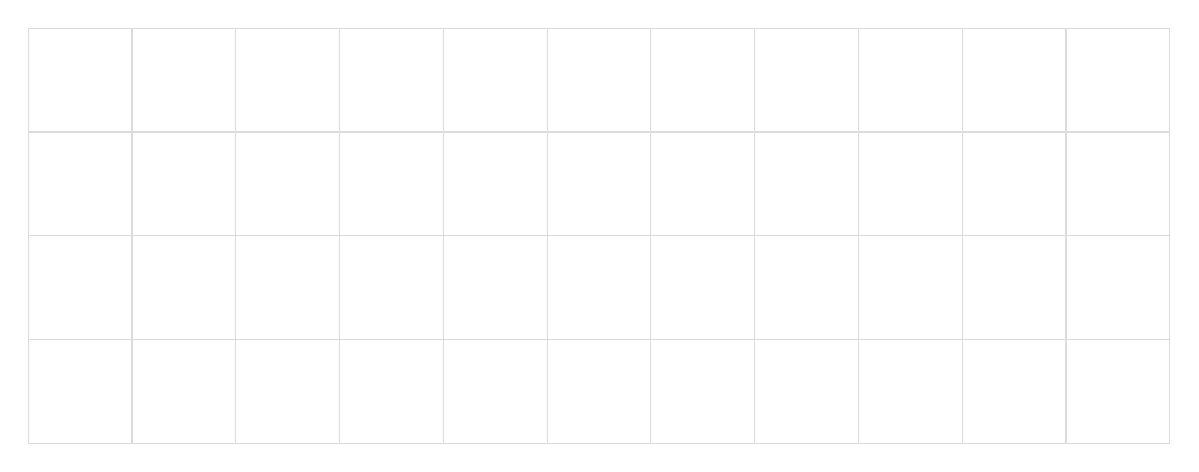
\begin{tikzpicture}[x=0.75pt,y=0.75pt,yscale=-1,xscale=1]
%uncomment if require: \path (0,208); %set diagram left start at 0, and has height of 208

%Shape: Grid [id:dp33505564538856114] 
\draw  [draw opacity=0] (2,2) -- (552,2) -- (552,202) -- (2,202) -- cycle ; \draw  [color={rgb, 255:red, 220; green, 220; blue, 220 }  ,draw opacity=1 ] (52,2) -- (52,202)(102,2) -- (102,202)(152,2) -- (152,202)(202,2) -- (202,202)(252,2) -- (252,202)(302,2) -- (302,202)(352,2) -- (352,202)(402,2) -- (402,202)(452,2) -- (452,202)(502,2) -- (502,202) ; \draw  [color={rgb, 255:red, 220; green, 220; blue, 220 }  ,draw opacity=1 ] (2,52) -- (552,52)(2,102) -- (552,102)(2,152) -- (552,152) ; \draw  [color={rgb, 255:red, 220; green, 220; blue, 220 }  ,draw opacity=1 ] (2,2) -- (552,2) -- (552,202) -- (2,202) -- cycle ;




\end{tikzpicture}

\fi

\section{Problem II}

Given $\bfvec{F}=3\ihat -4\jhat$, find

\begin{enumerate}

  \item Draw $\bfvec{F}$.

  \item Compute $F$.

  \item The angle  $\bfvec{F}$ makes with respect to the $x$--axis (with positive rotation counterclockwise).

\end{enumerate}

\ifsolutions
    \begin{enumerate}

      \item[2.] $F=\sqrt{3^2+4^2}=5$

      \item[3.] $\theta = 360^\circ - \tan^{-1}(4/3)\simeq 307^\circ$

    \end{enumerate}
\else



\tikzset{every picture/.style={line width=0.75pt}} %set default line width to 0.75pt        

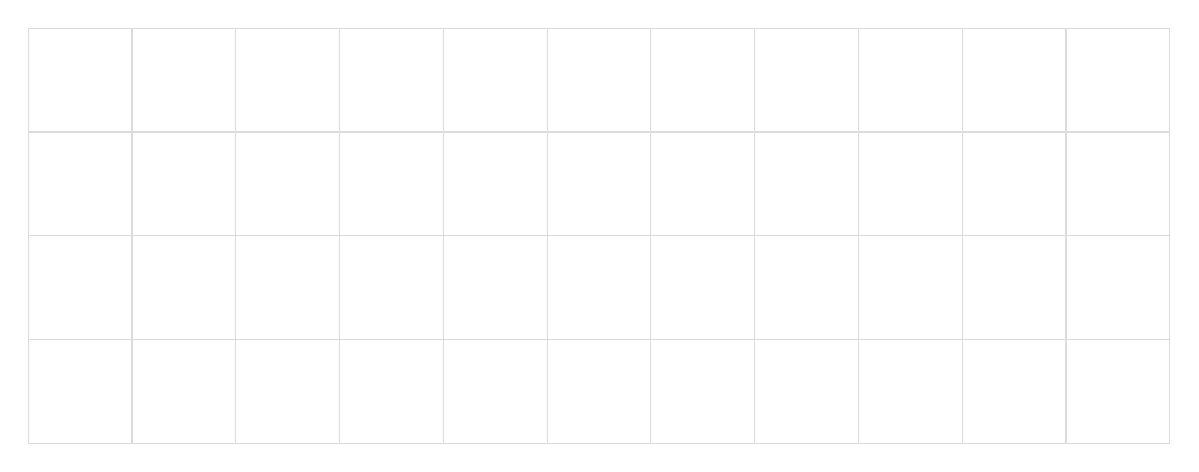
\begin{tikzpicture}[x=0.75pt,y=0.75pt,yscale=-1,xscale=1]
%uncomment if require: \path (0,208); %set diagram left start at 0, and has height of 208

%Shape: Grid [id:dp33505564538856114] 
\draw  [draw opacity=0] (2,2) -- (552,2) -- (552,202) -- (2,202) -- cycle ; \draw  [color={rgb, 255:red, 220; green, 220; blue, 220 }  ,draw opacity=1 ] (52,2) -- (52,202)(102,2) -- (102,202)(152,2) -- (152,202)(202,2) -- (202,202)(252,2) -- (252,202)(302,2) -- (302,202)(352,2) -- (352,202)(402,2) -- (402,202)(452,2) -- (452,202)(502,2) -- (502,202) ; \draw  [color={rgb, 255:red, 220; green, 220; blue, 220 }  ,draw opacity=1 ] (2,52) -- (552,52)(2,102) -- (552,102)(2,152) -- (552,152) ; \draw  [color={rgb, 255:red, 220; green, 220; blue, 220 }  ,draw opacity=1 ] (2,2) -- (552,2) -- (552,202) -- (2,202) -- cycle ;




\end{tikzpicture}

\fi

\end{document}